%%%%%%%%%%%%%%%%%%%%%%%%%%%%%%%%%%%%%%%%%
% a0poster Landscape Poster
% LaTeX Template
% Version 1.0 (22/06/13)
%
% The a0poster class was created by:
% Gerlinde Kettl and Matthias Weiser (tex@kettl.de)
%
% This template has been downloaded from:
% http://www.LaTeXTemplates.com
%
% License:
% CC BY-NC-SA 3.0 (http://creativecommons.org/licenses/by-nc-sa/3.0/)
%
%%%%%%%%%%%%%%%%%%%%%%%%%%%%%%%%%%%%%%%%%

%----------------------------------------------------------------------------------------
%	PACKAGES AND OTHER DOCUMENT CONFIGURATIONS
%----------------------------------------------------------------------------------------

\documentclass[a0,landscape]{a0poster}

\usepackage{multicol} % This is so we can have multiple columns of text side-by-side
\columnsep=80pt % This is the amount of white space between the columns in the poster
\columnseprule=3pt % This is the thickness of the black line between the columns in the poster

\usepackage[svgnames]{xcolor} % Specify colors by their 'svgnames', for a full list of all colors available see here: http://www.latextemplates.com/svgnames-colors

\usepackage{times} % Use the times font
%\usepackage{palatino} % Uncomment to use the Palatino font

\usepackage{graphicx} % Required for including images
\graphicspath{{figures/}} % Location of the graphics files
\usepackage{booktabs} % Top and bottom rules for table
\usepackage[font=small,labelfont=bf]{caption} % Required for specifying captions to tables and figures
\usepackage{amsfonts, amsmath, amsthm, amssymb} % For math fonts, symbols and environments
\usepackage{wrapfig} % Allows wrapping text around tables and figures
\usepackage[utf8]{inputenc} % Pour utiliser les caractères accentués
\usepackage{tikz}
\usetikzlibrary{shapes,snakes}
\usetikzlibrary{positioning}
\usepackage[export]{adjustbox}
\usepackage[skins,listings,breakable,listingsutf8,theorems,hooks,fitting]{tcolorbox}
\tcbuselibrary{raster}
\begin{document}

%----------------------------------------------------------------------------------------
%	POSTER HEADER
%----------------------------------------------------------------------------------------

% The header is divided into three boxes:
% The first is 55% wide and houses the title, subtitle, names and university/organization
% The second is 25% wide and houses contact information
% The third is 19% wide and houses a logo for your university/organization or a photo of you
% The widths of these boxes can be easily edited to accommodate your content as you see fit

\noindent\begin{minipage}[b]{\linewidth}
\centering
\noindent \veryHuge \color{NavyBlue} \textbf{Lake-river and lake-atmosphere interactions in a changing climate over Northeast Canada} \color{Black}\\ % Title
\noindent\begin{minipage}[c]{0.2\linewidth}
      \center
      
\includegraphics[width=25cm]{logo_cnrcwp_escer.png} % Logo or a photo of you, adjust its dimensions here
\end{minipage} \hfill
%
\begin{minipage}[c]{0.15\linewidth}
  \center
  \Large \textbf{Oleksandr Huziy} \\
  \large \texttt{guziy.sasha@gmail.com}
\end{minipage}
%
\begin{minipage}[b]{0.01\linewidth}
 \center
 \Large\&
\end{minipage}
%
\begin{minipage}[c]{0.15\linewidth}
   \center
   \Large \textbf{Laxmi Sushama} \\
   \large  \texttt{sushama.laxmi@uqam.ca}
\end{minipage}\hfill
%
\begin{minipage}[c]{0.2\linewidth}
  \center
  
\includegraphics[width=15cm]{logo_uqam.png} % Logo or a photo of you, adjust its dimensions here
\end{minipage}
\rule{\linewidth}{3pt}
\end{minipage}
%

\vspace{0.5cm} % A bit of extra whitespace between the header and poster content

%----------------------------------------------------------------------------------------

\begin{multicols}{3} % This is how many columns your poster will be broken into, a poster with many figures may benefit from less columns whereas a text-heavy poster benefits from more

%----------------------------------------------------------------------------------------
%	INTRODUCTION
%----------------------------------------------------------------------------------------

\color{SaddleBrown} % SaddleBrown color for the introduction

\section*{(A) Introduction}
Lakes influence the regional climate and hydrology in a number of ways and
therefore they should be represented in climate models in a realistic manner.
Lack of representation of lakes in models can lead to errors in simulated energy
and water fluxes, for lake-rich regions. This study focuses on the assessment of
the impact of climate change on lakes and hydrology as well as on the influence
of lakes on projected changes to regional climate and surface hydrology,
particularly streamflows, for Northeast Canada. To this end, transient climate
change simulations spanning the 1950--2100 period are performed, with and without
lakes, with the fifth generation of the Canadian Regional Climate Model (CRCM5),
driven by the Canadian Earth System Model (CanESM2) at the lateral boundaries
for Representative Concentration Pathway 8.5.

%----------------------------------------------------------------------------------------
%	OBJECTIVES
%----------------------------------------------------------------------------------------

\color{DarkSlateGray} % DarkSlateGray color for the rest of the content

\section*{(B) Main Objectives}
\begin{tcolorbox}[colback=white,colframe=green!40!black]
  \begin{enumerate}
  \item Improve most important processes essential for simulating streamflow (rivers, river-lake connectivity, etc).
  \item Study/quantify atm.-lake-river interactions through carefully designed experiments.
  \item Study/quantify impact of lake-atmosphere, of lake-river interactions on the projected changes to selected hydrological/near-surface climate variables over northeastern Canada.
  \end{enumerate}
\end{tcolorbox}

%----------------------------------------------------------------------------------------
%	MATERIALS AND METHODS
%----------------------------------------------------------------------------------------

\section*{(C) Methods and experiment configurations}
\subsection*{C.1 Methods}
%
The impacts of lake-atmosphere interactions on
projected changes and the impacts of direct lake-river interactions on projected
changes in streamflow are assessed using the configurations with and without
lakes, described below.\\[0.5cm]

\begin{minipage}[t]{\linewidth}
\small
\begin{tabular}{lll}
\toprule
\textbf{Simulation} & \textbf{Period} & \textbf{Description}\\
\midrule
ERAI-CRCM5-NL     & 1979--2010 & Reanalysis-driven, lakes are replaced with bare ground \\
ERAI-CRCM5-L1     & 1979--2010 & Reanalysis-driven, includes lake-atm. interactions, but no lake-river interactions\\
ERAI-CRCM5-L      & 1979--2010 & Reanalysis-driven, includes lake-atm. and lake-river interactions\\
CanESM2-CRCM5-NL & 1950--2100 & CanESM2-driven, lakes are replaced with bare ground \\
CanESM2-CRCM5-L  & 1950--2100 & CanESM2-driven, includes lake-atm. and lake-river interactions \\
\bottomrule
\end{tabular}
\captionof{table}{\color{Green} List of simulations used in the current study}
\end{minipage}

%
\begin{minipage}[t]{\linewidth}
\flushleft
\begin{tikzpicture}
    % schematics
    \node[label={\small NL (no lakes)}] (nl) at (0,0) {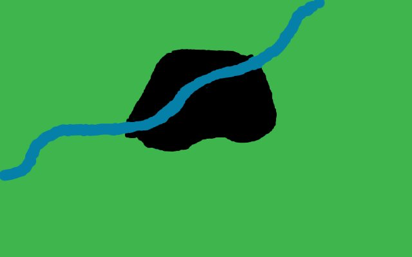
\includegraphics[scale=0.5]{crcm5-nl}};
    \node[label={\small L (with lakes)}] (wl) at (0,-5) {
\includegraphics[scale=0.5]{crcm5-l}};

    \node (middle) at (6, -2.5) {};

    % lines
    \draw[line width=5pt] (nl.east) -- (middle.west);
    \draw[line width=5pt] (wl.east) -- (middle.west);

    % explanation bullets
    \node[text width=0.7\linewidth, draw] (b1) at (18, -1) {$\bullet$ By comparing projected changes to atmospheric fields \\ $\longrightarrow$ Impact of lake-atm. interactions.};
    \node[text width=0.7\linewidth, draw] (b2) at (18, -4) {$\bullet$ By comparing projected changes to streamflow \\ $\longrightarrow$ Direct \& indirect impact of lakes on changes to streamflow.};
\end{tikzpicture}
\end{minipage}


\subsection*{C.2 Experiment setup}

\begin{tcolorbox}[colback=white,colframe=green!40!black]
\begin{minipage}{0.48\linewidth}
\begin{itemize}
  \item Horizontal grid: 260$\times$260, \color{Red} dx=0.1$^\circ$ \color{DarkSlateGray};
  \item Time step: \color{Red} 5 min \color{DarkSlateGray};
  \item Analysis periods: \\ \textbf{1980--2010} and \textbf{2070--2100};
  \item Surface scheme: CLASS3.5;
\end{itemize}
\end{minipage} \hfill
%
\begin{minipage}{0.48\linewidth}
\begin{itemize}
  \item Lake model: Hostetler;
  \item River model: WATROUTE-modified;
  \item Lateral boundary conditions:
    \begin{itemize}
        \item ERA-Interim, 1.5$^\circ$
        \item CanESM2 outputs
    \end{itemize}
\end{itemize}
\end{minipage}
\end{tcolorbox}

\begin{minipage}[c]{\linewidth}
  \center
  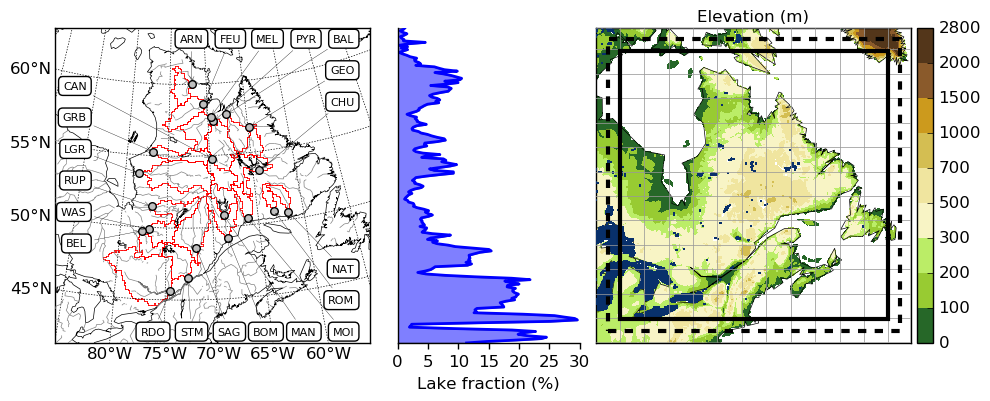
\includegraphics[width=0.7\linewidth]{qc_basin_outlets_points}
  \captionof{figure}{\color{Green} Left panel: domain with basins of interest, the grey circles show basin outlets determined from the flow
  direction field, used for streamflow simulations; middle panel: zonally averaged lake fractions. Right panel: topography [m], the cells with lake fractions greater or equal to 0.6 are indicated with blue colour,
  the gray cells contain 20$\times$20 grid cells.}
\end{minipage}

%----------------------------------------------------------------------------------------
%	RESULTS
%----------------------------------------------------------------------------------------

\section*{(D) Results}

\subsection*{D.1 Validation}
\begin{minipage}[c]{0.45\linewidth}
\begin{center}
  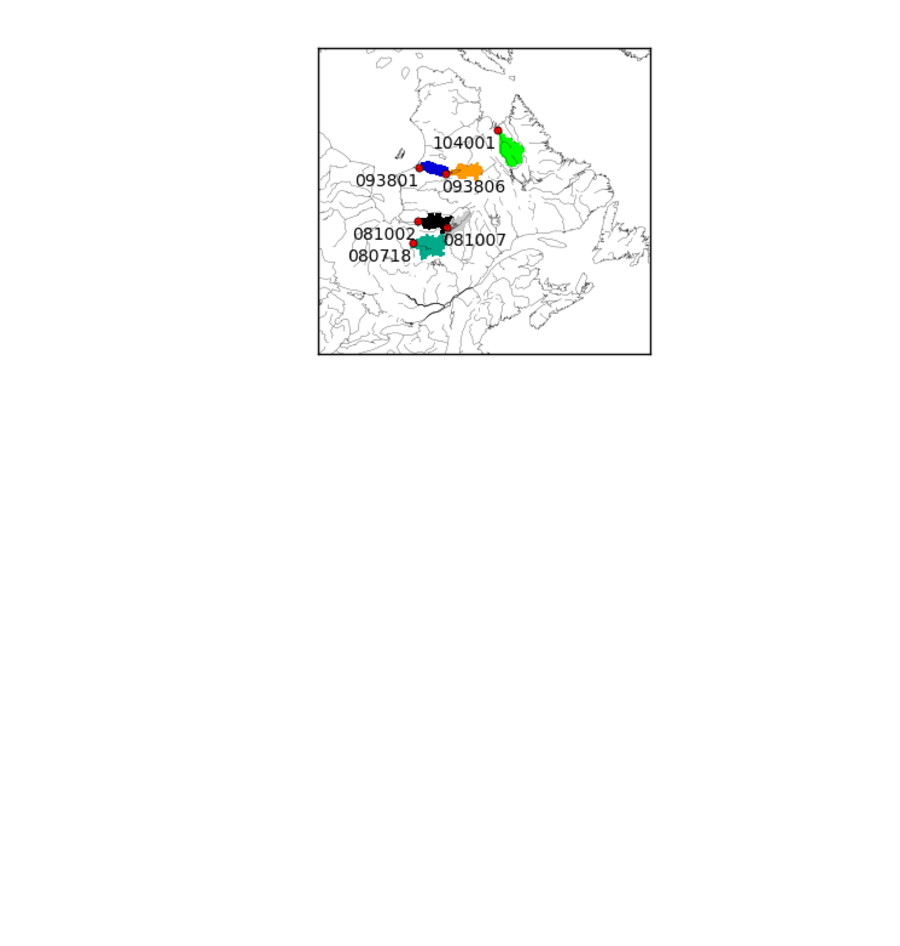
\includegraphics[width=0.6\linewidth]{streamflow_validation_6_positions}
  \captionof{figure}{\color{Green} Locations and identification numbers (IDs) of the selected gauging stations
with their upstream areas (determined from the flow directions field) shown
shaded.}
\end{center}
\end{minipage}\hfill
%
\begin{minipage}[c]{0.50\linewidth}
\begin{center}
  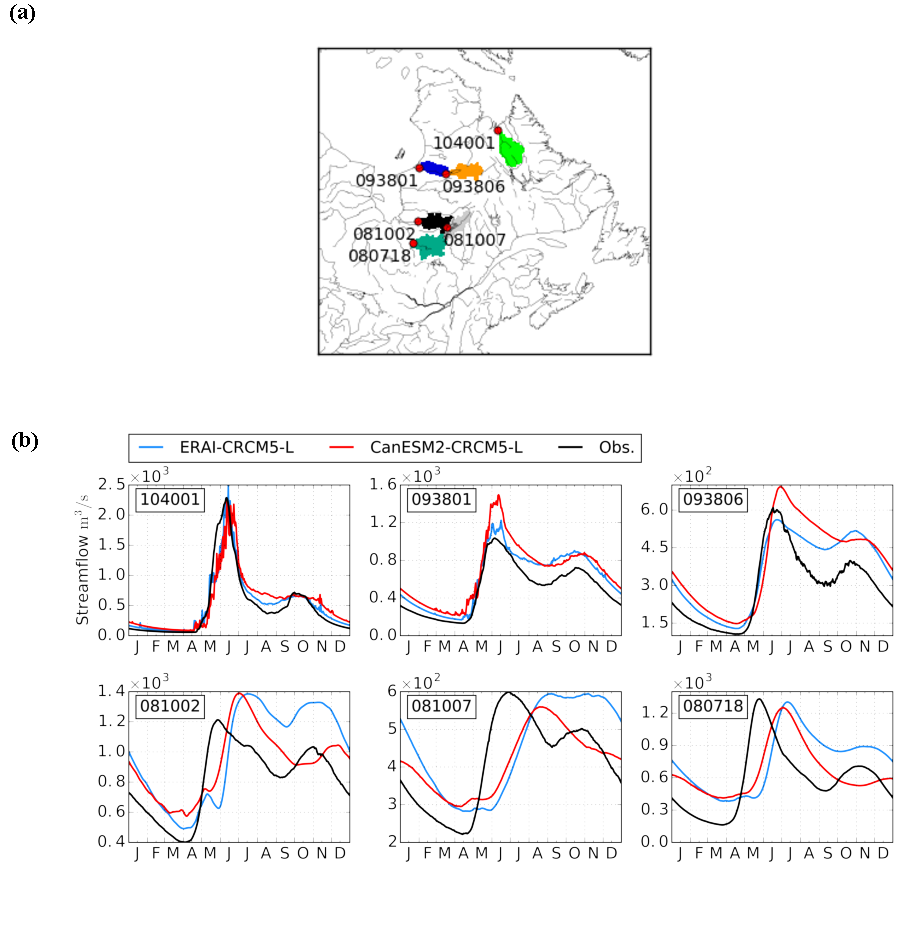
\includegraphics[width=0.95\linewidth]{streamflow_validation_6}
  \captionof{figure}{\color{Green} Comparison of observed (black) and modelled (blue and red correspond
to ERAI-CRCM5-L and CanESM2-CRCM5-L simulations, respectively) daily
climatological streamflow [m$^3$/s] at selected stations. }
\end{center}
\end{minipage}
%
\begin{tcolorbox}[colback=white,colframe=green!40!black]
\begin{itemize}
  \item Simulated streamflow mostly compares reasonably with the observations
  \item The lower performance for the southern stations is due to the uncertainties in soil parameters, which leads to higher infiltration during melting period and streamflow overestimation afterwards.
\end{itemize}
\end{tcolorbox}

\subsection*{D.2 Impacts of lake-atmosphere and lake-river on simulated mean streamflows: 1980--2010 period, m$^3$/s}

\begin{minipage}{\linewidth}
  \center
  \begin{tikzpicture}
      % impacts of lake-atm. and lake-river interactions in current climate
      \node[label={\small ERAI-CRCM5-L1 minus ERAI-CRCM5-NL}] (la) at (-9,0) {
        \adjincludegraphics[trim={{0.125\width} {0.35\height} {0.105\width} {0.5\height}}, clip]{STFA_CRCM5-L1_CRCM5-NL}};
      \node[label={\small ERAI-CRCM5-L minus ERAI-CRCM5-L1}] (lr) at (9,0) {
        \adjincludegraphics[trim={{0.125\width} {0.35\height} {0.105\width} {0.5\height}}, clip]{STFA_CRCM5-L2_CRCM5-L1}};
  \end{tikzpicture}
  \captionof{figure}{\color{Green} Impacts of lake-atm. interactions (left) and impacts of lake-river interactions (right). Not significant impacts are shown in gray.}
\end{minipage}


\begin{tcbitemize}[raster columns=2, raster equal height]
%\tcbitem[colback=white,colframe=white,sidebyside align=top,sidebyside]
  \tcbitem[colback=white,colframe=green!40!black, adjusted title={Lake-atm. interactions}]
  \begin{itemize}
    \item Impact of lake-atm. interactions is mostly positive, but modest.
  \end{itemize}

\tcbitem[colback=white,colframe=green!40!black, adjusted title={Lake-river interactions}]
  \begin{itemize}
    \item Winter impacts are positive and significant for the bigger northern part of the domain due to additional water coming to the river network from lakes.
    \item Mostly negative impacts are obtained in spring since part of water from snow melt is stored in lakes to be released later into the river network.
  \end{itemize}

\end{tcbitemize}


\subsection*{D.3 Impacts of lake-atmosphere and lake-river interactions on projected climate changes}
\begin{minipage}[t]{\linewidth}
\center
\begin{tikzpicture}
    % schematics
    \node[label={\small CanESM2-CRCM5-L (with lakes)}] (lcc) at (0,0) {\includegraphics[scale=0.65]{cc_seasonal_with_lakes}};
    \node[label={\small CanESM2-CRCM5-NL (no lakes)}] (nlcc) at (20,0) {\includegraphics[scale=0.65]{cc_seasonal_no_lakes}};
    \node[diamond, text width=0.05\linewidth, align=center, draw] (operation) at (10,-7.5) {\Huge -};

    \node[label={\small CanESM2-CRCM5-L minus CanESM2-CRCM5-NL}] (lcc_vs_nlcc) at (20,-18) {\includegraphics[scale=0.7]{impact_of_lakes_on_cc}};

    % lines
    \draw[-latex, line width=5pt] (operation.south) to[out=-90,in=180] (lcc_vs_nlcc.west);
    \draw[-latex, line width=5pt] (lcc.south) to[out=-30,in=180] (operation.west);
    \draw[-latex, line width=5pt] (nlcc.south) to[out=-150,in=0] (operation.east);

    %Points
    \node[draw, text width=0.5\linewidth] (point1) at (0, -10.5) {$\bullet$ Lakes attenuate projected changes to the temperature during all seasons};
    \node[below= 0.5cm of point1, draw, text width=0.5\linewidth] (point2) {$\bullet$ Attenuated precipitation increases in winter and spring are due to attenuated increases in temperature by lakes};
    \node[below=0.5cm of point2, draw, text width=0.5\linewidth] (point3) {$\bullet$ Decreases in SWE are amplified by lakes in the northern part in winter and spring due to attenuated increases in precipitation};
    \node[below=0.5cm of point3, draw, text width=0.5\linewidth] (point4) {$\bullet$ Lakes mostly dampen amplitudes of projected increases and decreases to streamflow};

    \node[below=1.0cm of point4, draw, text width=0.5\linewidth, align=left] (winter){\small \textbf{Winter streamflow.} Dipole pattern: \color{Blue}negative \color{DarkSlateGray} sign due to meltwater stored in lakes, \color{Red}positive \color{DarkSlateGray} sign since lakes supply water in frozen conditions};
    \node[below=1.0cm of lcc_vs_nlcc, draw, text width=0.5\linewidth, align=left] (summer){\small \textbf{Summer streamflow.} Decreases in streamflow are dampened by additional water from lakes};


    %lines streamflow
    \draw[-latex, line width=5pt] (winter.east) to[out=0,in=215] ([xshift=2em,yshift=1.5em]lcc_vs_nlcc.south west);
    \draw[-latex, line width=5pt] ([xshift=-0.5em]summer.north) to[out=90,in=215] ([xshift=0.5em,yshift=1.5em]lcc_vs_nlcc.south);


\end{tikzpicture}
\end{minipage}



%----------------------------------------------------------------------------------------
%	CONCLUSIONS
%----------------------------------------------------------------------------------------

\color{SaddleBrown} % SaddleBrown color for the conclusions to make them stand out

\section*{(E) Conclusions}

\begin{itemize}
\item Comparison of projected changes from the simulations with and without lakes suggests important impact of lakes on projected increases to 2-m temperatures, due to thermal inertia of lakes.
\item Amplitudes of projected changes to streamflows are mostly dampened by lake-river interactions. Although a north-south dipole pattern, due to frozen conditions, can be noted in winter.
\end{itemize}

\color{DarkSlateGray} % Set the color back to DarkSlateGray for the rest of the content


 %----------------------------------------------------------------------------------------
%	REFERENCES
%----------------------------------------------------------------------------------------

\nocite{*} % Print all references regardless of whether they were cited in the poster or not
\small
\bibliographystyle{plain} % Plain referencing style
\bibliography{sample} % Use the example bibliography file sample.bib

%----------------------------------------------------------------------------------------
%	ACKNOWLEDGEMENTS
%----------------------------------------------------------------------------------------
\section*{Acknowledgements}
\small
This research was carried out within the Canadian Network for Regional Climate and Weather Processes (CNRCWP) project funded by the Natural Sciences and Engineering Research Council (NSERC) of Canada.
%----------------------------------------------------------------------------------------

\end{multicols}
\end{document}
